\documentclass[12pt]{article}
\usepackage{xeCJK}
\usepackage{tikz}
\usepackage{ifthen}
\usepackage{intcalc}
\usetikzlibrary{calc}
\setCJKmainfont{NotoSerifTC-Regular.otf}
\title{DAU Figures}
\author{Chen, Chao-Ting}

\begin{document}
\maketitle

\begin{figure}
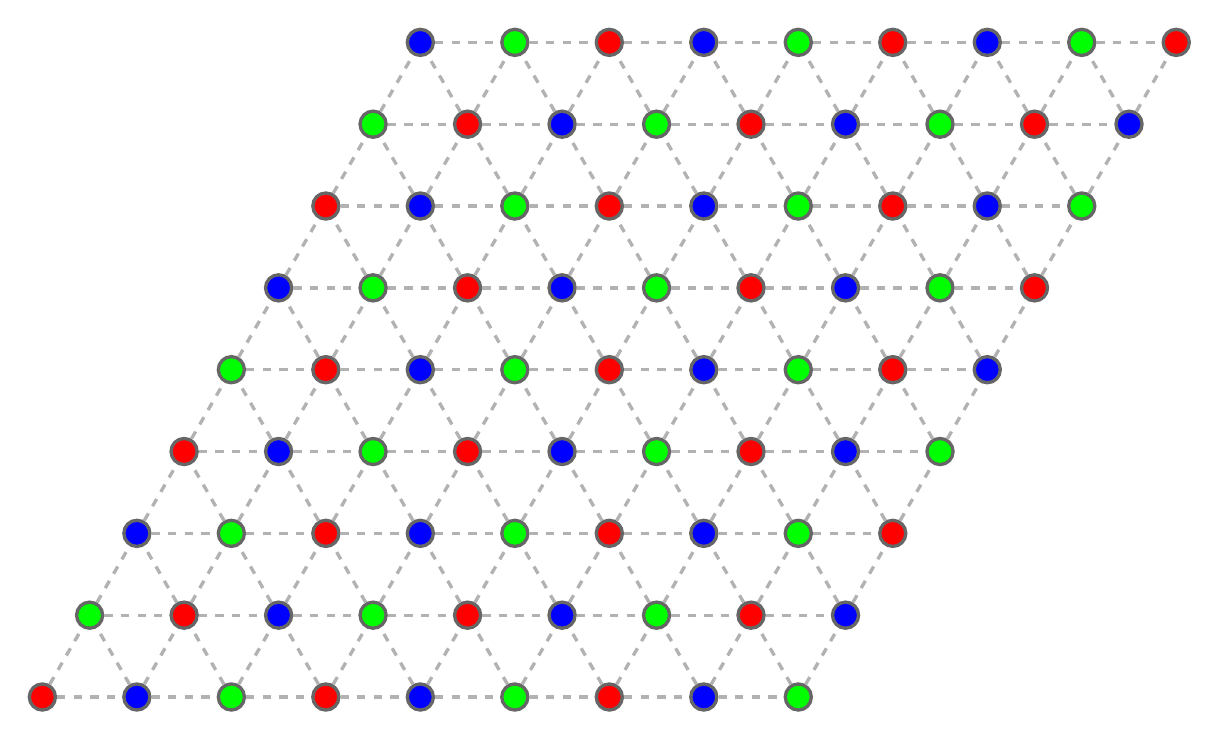
\begin{tikzpicture}[
    roundnode/.style={circle, draw=black!60, very thick, minimum size=3mm},
]   
    \NewExpandableDocumentCommand{\sqrtVal}{O{16}m}{%
    \fpeval{round(sqrt(#2),#1)}%
    }
    
    % the start coordinate
    \coordinate (start) at (0, 0) ;
    
    % the lattices
    \foreach \i in {0, ..., 8}
    {
        % \node at (\x, 1) [roundnode, fill=red!100](dot){} ;
        \foreach \j in {0, ..., 8}
        {
            % coordinate color: 
            % 2*i + j = 0 => red
            \def\xycondition{\intcalcMod{2*\i+\j}{3}}
            \ifthenelse{ \xycondition = 0 }
                { \def\nodecolor{red} }
            {
                % 2*i + j = 1 => blue
                % 2*i + j = 2 => green
                \ifthenelse{ \xycondition = 1 } 
                    { \def\nodecolor{blue} }
                    { \def\nodecolor{green} }
            }

            % x: i/2 + j 
            % y: sqrt(3) * i/2 
            \node at ($(start) + 1.2*( \i/2+\j, \sqrtVal{3}/2*\i )$) 
            [
                roundnode,
                % color  
                fill=\nodecolor!100,
            ](roundnode_\i_\j){} ;
            
        }
    }

    \foreach \i in {0, ..., 7}
    {
        \foreach \j in {0, ..., 7}
        {
            \draw [very thick, dashed, draw=gray!60] (roundnode_\i_\j) -- (roundnode_\i_\fpeval{\j+1}) ;
            \draw [very thick, dashed, draw=gray!60] (roundnode_\i_\j) -- (roundnode_\fpeval{\i+1}_\j) ;
        }
        \draw [very thick, dashed, draw=gray!60] (roundnode_8_\i) -- (roundnode_8_\fpeval{\i+1}) ;
        \draw [very thick, dashed, draw=gray!60] (roundnode_\i_8) -- (roundnode_\fpeval{\i+1}_8) ;
    }

    \foreach \i in {0, ..., 7}
    {
        \foreach \j in {1, ..., 8}
        {
            \draw [very thick, dashed, draw=gray!60] (roundnode_\i_\j) -- (roundnode_\fpeval{\i+1}_\fpeval{\j-1}) ;
        }
    }

\end{tikzpicture}
\caption{Triangular Lattice} \label{fig:Triangular Lattice}
\end{figure}

\begin{figure}
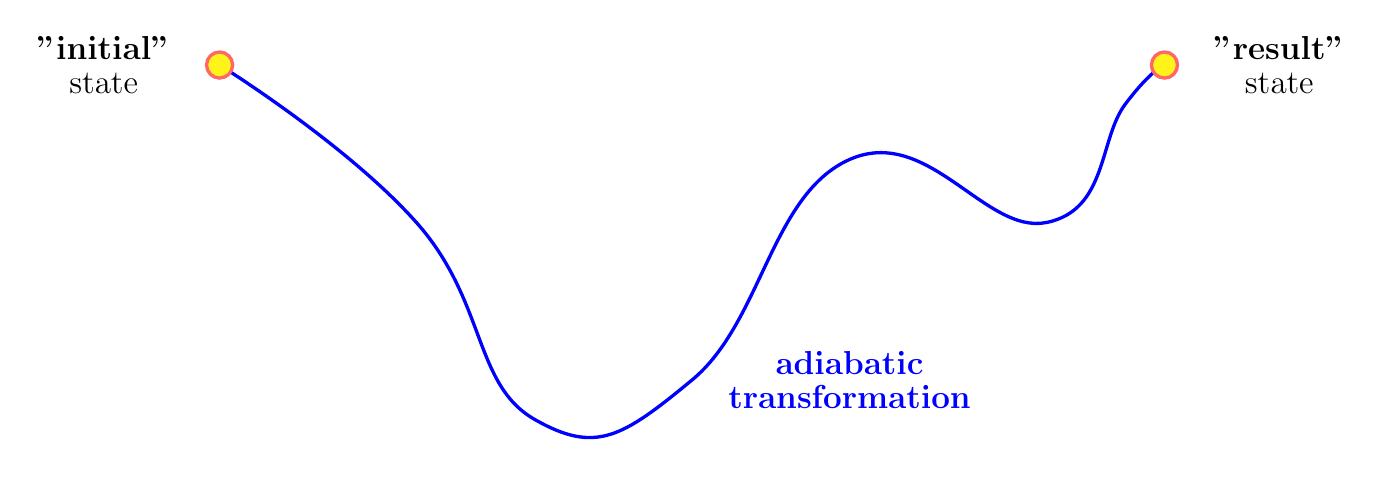
\begin{tikzpicture}[
    roundnode/.style={circle, draw=red!60, fill=yellow!90, very thick, minimum size=3mm},
]
    % \draw [gray!50]  
    % (0,0) -- (2.5,-1.5) -- (4,-4.5) -- (7,-3.5) -- (8,-1.5) -- (9,-2) -- (11.5,-0.2) -- (12,0);
    \draw [blue, very thick] plot [smooth, tension=0.8] coordinates 
    { (0,0) (2.5,-2) (4,-4.5) (6,-4) (8,-1.2) (10.5,-2) (11.5,-0.5) (12,0) };
    
    \node at (0, 0) [roundnode ](start){} ;
    \node at (12, 0) [roundnode ](end){} ;

    \node at ($(start) + (-0.5, 0)$) [align=center, anchor=east](){\large \textbf{"initial"} \\ \large state} ;
    \node at ($(end) + (0.5, 0)$) [align=center, anchor=west](){\large \textbf{"result"} \\ \large state} ;
    \node at (8, -4) [align=center, blue](){\large \textbf{adiabatic} \\ \large \textbf{transformation} } ;

\end{tikzpicture}
\caption{Adiabatic Quantum Computing} \label{fig:Adiabatic Quantum Computing}
\end{figure}

\begin{figure}
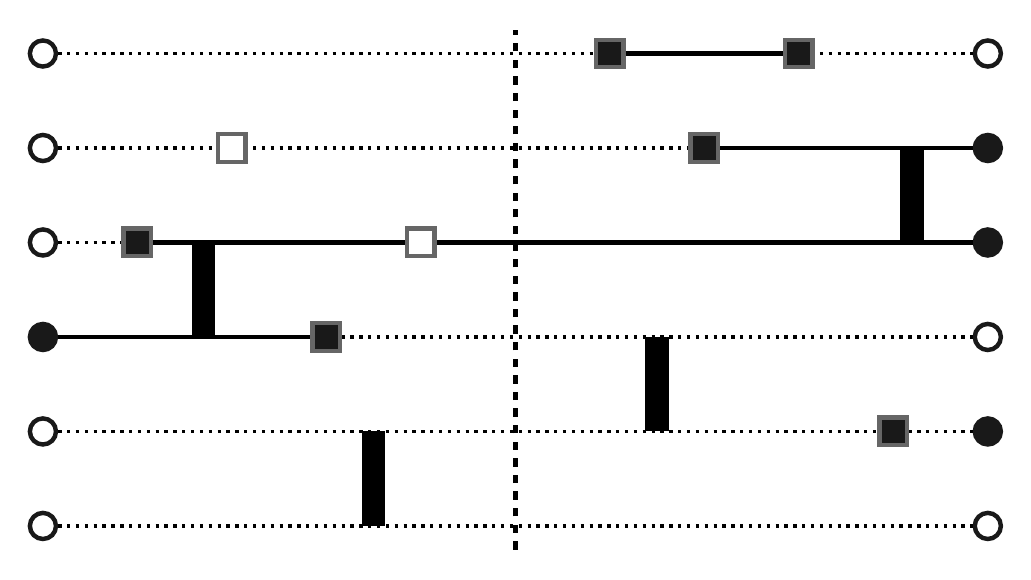
\begin{tikzpicture}[
    roundnode/.style={circle, draw=black!90, ultra thick, minimum size=3mm},
    rectnode/.style={rectangle, draw=black!60, ultra thick, minimum size=3.5mm}, 
]
    
    \def\xScale{1.2}
    \def\yScale{1.2}
    
    % left white nodes
    \foreach \i in {1, 2, 4, 5, 6}
    {
        \node at (0, 1.2*\i) [roundnode, fill=white!90](Lcircle_\i){};
    }

    % left black nodes
    \foreach \i in {3}
    {
        \node at (0, 1.2*\i) [roundnode, fill=black!90](Lcircle_\i){};
    }

    % right white nodes
    \foreach \i in {1, 3, 6}
    {
        \node at (10*\xScale, \i*\yScale ) [roundnode, fill=white!90](Rcircle_\i){};
    }

    % right black nodes
    \foreach \i in {2, 4, 5}
    {
        \node at (10*\xScale, \i*\yScale ) [roundnode, fill=black!90](Rcircle_\i){};
    }

    % connect the horizon line of six nodes
    \foreach \i in {1, ..., 6}
    {
        \draw [very thick, dotted] (Lcircle_\i) -- (Rcircle_\i) ;
    }

    % the middle vertical line (the check section)
    \def\Yshift{0.3}
    \draw [ultra thick, dashed] (6, 1.2 - \Yshift) -- (6, 1.2*6 + \Yshift) ;
    
    % black gates
    \foreach \i/\j/\posX in {
    % square black node: (invert gate) 
    % i:    the i line from bottom,  
    % j:    the j gate from left,
    % posX: the posX is the gate position on that line
    2/1/9,
    3/1/3, 
    4/1/1, 
    5/2/7, 
    6/1/6, 
    6/2/8}
    {
        \node [rectnode, fill=black!90] at (\posX*\xScale, \i*\yScale ) (gate_\i_\j){};
    }

    % white gates
    \foreach \i/\j/\posX in {
    % square white node: (non-change gate) 
    % i:    the i line from bottom,  
    % j:    the j gate from left,
    % posX: the posX is the gate position on that line
    4/2/4,
    5/1/2}
    {
        \node [rectnode, fill=white!90] at (\posX*\xScale, \i*\yScale ) (gate_\i_\j){};
    }

    % horizontal gate inverted part
    \foreach \start/\end in {
    Lcircle_3/gate_3_1,
    gate_4_1/gate_4_2,
    gate_4_2/Rcircle_4,
    gate_5_2/Rcircle_5,
    gate_6_1/gate_6_2}
    {
        \draw [ultra thick] (\start) -- (\end) ;
    }

    % horizontal gate connect part
    \foreach \x/\downY/\upY in {
    3.5/1/2,
    6.5/2/3,
    1.7/3/4,
    9.2/4/5}
    {
        % (10*\xScale, \i*\yScale )
        \draw [ultra thick, line width=3mm] (\x*\xScale, \downY*\yScale ) -- (\x*\xScale, \upY*\yScale ) ;
    }

\end{tikzpicture}
\caption{Projector QMC} \label{fig:Projector QMC}
\end{figure}

\end{document}